\documentclass[11pt,a4paper]{article}
\usepackage{fontspec}
\setmainfont{TeX Gyre Pagella}
\newfontfamily\headfont{Inter}[UprightFont=*-ExtraBold,BoldFont=*-ExtraBold,Extension=.otf,Path=/usr/share/fonts/opentype/inter/]
\usepackage[a4paper,margin=2.3cm]{geometry}
\usepackage{graphicx,booktabs,float,caption,array,xcolor,longtable}
\usepackage{xurl}
\usepackage[hidelinks]{hyperref}
\usepackage{titlesec}
\usepackage[round]{natbib}
\usepackage{setspace}
\setstretch{1.05}
\renewcommand{\topfraction}{0.9}
\renewcommand{\bottomfraction}{0.8}
\renewcommand{\textfraction}{0.1}
\renewcommand{\floatpagefraction}{0.75}
\setlength{\parindent}{0pt}
\setlength{\parskip}{0.55em}
\titleformat{\section}{\headfont\Large}{\thesection}{0.8em}{}
\titleformat{\subsection}{\headfont\large}{\thesubsection}{0.8em}{}
\captionsetup{font=small,labelfont=bf}
\urlstyle{same}
\hypersetup{pdftitle={Lost at Sea: Famous Disappearances Tested against Shipping Traffic},pdfauthor={Tristan Hotham}}

\begin{document}
\begin{center}
{\Large\bfseries Lost at Sea: Famous Disappearances Tested against Shipping Traffic\par}
\vspace{0.4em}
{\large Is the Bermuda Triangle, or anywhere else, worse than its traffic would predict?\par}
\vspace{1.2em}
{\large Tristan Hotham\par}
\vspace{0.3em}
{\small Independent researcher\\
ORCID: 0000-0003-4931-9349\\
DOI: https://doi.org/10.5281/zenodo.23856868\par}
\vspace{0.8em}
2026
\end{center}

\begin{quote}
\small
\begin{center}\textbf{Abstract}\end{center}
The Bermuda Triangle is said to claim more ships and aircraft than its traffic can explain. I test that claim, and the same claim for every other sea, with open data. From Wikipedia's lists of missing ships, missing aircraft and people who disappeared mysteriously at sea, and the articles on the Bermuda, Dragon's and Michigan Triangles, I built a catalogue of 673 famous disappearances and placed 472 of them at sea from their location text. I compared 27 sea areas, and 2 degree squares, with modern shipping (the World Bank and IMF's AIS ship density, 2015 to 2021) and with 17,224 recorded wrecks that have a position. The Bermuda Triangle holds 8 placed disappearances against 2.8 expected from its traffic (2.9 times; 95\% interval 1.2 to 5.6), but its four neighbouring seas have the same excess (2.7 times), and within that group the Triangle holds exactly its share (8 against 7.7). Only 2 of the 14 incidents told in its Wikipedia article lie inside the triangle as usually drawn. The Dragon's Triangle is as expected and the Michigan Triangle holds none. The seas that really are worse than their traffic are Bass Strait and the Tasman Sea, the Great Lakes, the English Channel, the US Atlantic coast, the Caribbean and the Grand Banks, and each has a plain explanation: weather, shoals, historical traffic, aviation and who wrote the losses down.

\textbf{Keywords:} Bermuda Triangle; disappearances at sea; shipping traffic; AIS; funnel plot; Poisson; Wikipedia; maritime history; open data
\end{quote}

\section{Introduction}
Since Vincent Gaddis gave the Bermuda Triangle its name and its vertices (Miami, San Juan and Bermuda) in a magazine article of 1964, and Charles Berlitz made it a best seller a decade later \citep{berlitz}, the claim has been that ships and aircraft vanish there more often than elsewhere \citep{wikibt}. The standard reply, made most fully by Larry Kusche \citep{kusche}, is that the area is busy, stormy and badly reported, and that many of its famous losses happened somewhere else. Both sides are making a quantitative claim about losses per unit of traffic, but neither had a map of traffic.

Such a map now exists. The World Bank and the IMF publish a global raster of ship density built from AIS position reports \citep{wbdensity,cerdeiro}. And Wikipedia's volunteers have compiled lists of missing ships, missing aircraft and people who disappeared mysteriously at sea, alongside the articles on the Bermuda Triangle and its two lesser cousins, the Dragon's Triangle (the Devil's Sea) south of Japan and the Lake Michigan Triangle \citep{wikimships,wikimair,wikipeople,wikids,wikilm}. This paper places those disappearances on the map and asks, for every sea: how many would we expect if disappearances simply followed traffic, and how many are there? An interactive version is at \url{https://maps.tristanhotham.com/lost-at-sea/}.

\section{Data}
\textbf{Famous disappearances.} I parsed the tables of the three Wikipedia lists, with row spans filled in: 201 rows of missing ships, 289 of missing aircraft and 223 incidents from the people list (rows that continue a row span, such as the second Vivaldi brother, are folded into one incident; the list's ``solved cases'' are left out). I added 21 incidents told in the three triangle articles, with positions read from the article text (for example ``wreck found 35 nmi off St.~Augustine'' for the Cotopaxi). Each row keeps its year and its location text. Wikipedia text is CC BY-SA 4.0; the derived catalogue is shared under the same licence.

\textbf{Shipping traffic.} The World Bank's Global Shipping Traffic Density \citep{wbdensity} counts AIS positions of all vessels from January 2015 to February 2021 on a 0.005 degree grid, produced by the IMF and World Bank from the AIS data behind \citet{cerdeiro}; it is CC BY 4.0. I used the 0.08 degree overview level of the published raster. That level was made by sampling single full-resolution pixels, so individual values are noisy; I only use sums over 2 degree squares (about 625 samples each) and over named seas (thousands). It is a proxy for modern traffic only.

\textbf{Recorded losses.} As a historical denominator I use the 17,224 wrecks with a position in two global records, as cleaned for an earlier study \citep{hotham}: entries of Wikipedia's ``List of shipwrecks'' pages that give coordinates (15,133; CC BY-SA 4.0) and Wikidata wrecks (2,091; CC0). Of these, 15,761 are dated 1800 to 2025 and 433 are dated 2000 to 2025. I left out the national bulk records in that study (Canmore for Scotland, Coflein for Wales, NOAA's AWOIS for the United States), which would make the seas of three countries look far more dangerous than all others. Natural Earth supplies coastlines \citep{naturalearth}.

\section{Methods}
\subsection{Placing the disappearances}
Each incident was placed from its location text with a hand-made gazetteer of 359 ports, capes, islands and coasts and 58 named seas, in four grades of confidence: \emph{position given} (coordinates, or a distance and bearing from a named place, 37 incidents); \emph{near a named place} (``off'', ``near'' or ``around'' a cape, island or port, 220); \emph{route midpoint} (``between A and B'' or ``from A to B'': the great-circle midpoint, for routes up to 4,000 km, 52); and \emph{sea area only} (a representative point inside a named sea, 163). Routes of 4,000 to 7,000 km (most of them transatlantic) count only for the open sea they cross. For the aircraft and people lists, the circumstances text was used only when the location column gave an ocean or nothing better. A point that fell on land was moved to the nearest sea within 75 km (200 km for routes); 42 were moved. Incidents placed only by a whole ocean, lost over land, or on routes that cross continents were left out: 201 of 673. 134 cases (including the 21 article incidents) were placed or corrected by hand, each with a note in the code.

Duplicates were merged when two rows shared a year and a distinctive name word (for the people list, also a capitalised word of the circumstances), or an aircraft and a person shared a full date and lay within 1,500 km, but never two differently named ships or aircraft. 61 rows were merged, leaving 673 incidents.

\subsection{Seas, squares and expected counts}
I drew 27 named areas as simple polygons, tested in order so that they never overlap: the three triangles (the Bermuda Triangle from Miami to Bermuda to San Juan; the Dragon's Triangle from Tokyo to Guam to Taipei, a generous version around the Wikipedia article's centre point, since the article says its outline varies by author; and the Michigan Triangle from Ludington to Manitowoc to Benton Harbor), then smaller seas, then larger ones, and the rest of the world's seas. Incidents placed only by a sea's name are never counted inside a triangle (the representative point of ``Lake Michigan'' happens to fall inside the Michigan Triangle, which would otherwise be credited with four incidents it does not own).

For area $a$ with traffic share $t_a$ and $N$ placed incidents, the expected count is $E_a = N t_a$ and the ratio is $O_a/E_a$. Intervals are exact Poisson 95\% intervals for $O_a$ \citep{garwood} divided by $E_a$. ``Clearly'' more or fewer means beyond the 99.8\% limit of a funnel plot \citep{spiegelhalter}, that is a one-sided Poisson probability below 0.001. I report four tests:
\begin{itemize}
\item \textbf{T}: disappearances against traffic, as above.
\item \textbf{L}: disappearances of 1800 to 2025 against recorded losses of 1800 to 2025, $E_a = N_{1800} \ell_a$, where $\ell_a$ is the area's share of recorded losses; and the same without the world-war years.
\item \textbf{M}: recorded losses of 2000 to 2025 against traffic, the closest match of eras.
\item \textbf{Sensitivities}: a ``lanes'' traffic index (the share of sampled pixels with at least 1,000 AIS positions), which is less sensitive to how densely receivers pick up ships; incidents since 1946 only; ships only; and incidents placed by a position or a named place only.
\end{itemize}
For 2 degree squares I use only incidents placed by a position, a named place or a route (309), and rank squares with at least two incidents beyond the 99.8\% limit.

\section{Results}
\subsection{The catalogue}
Of the 472 placed incidents, 174 are ships and boats, 180 aircraft and 118 people lost from a vessel or with one. Their median year is 1940; 69\% are from before 1946 and 25\% from the two world wars (Figure~\ref{fig:decades}). Their map (Figure~\ref{fig:map}) already shows the shape of the result: dense clusters off North America, around Britain, in Bass Strait and the Great Lakes, and very few off East Asia, whose shipping lanes are among the busiest in the world.

\begin{figure}[tbp]\centering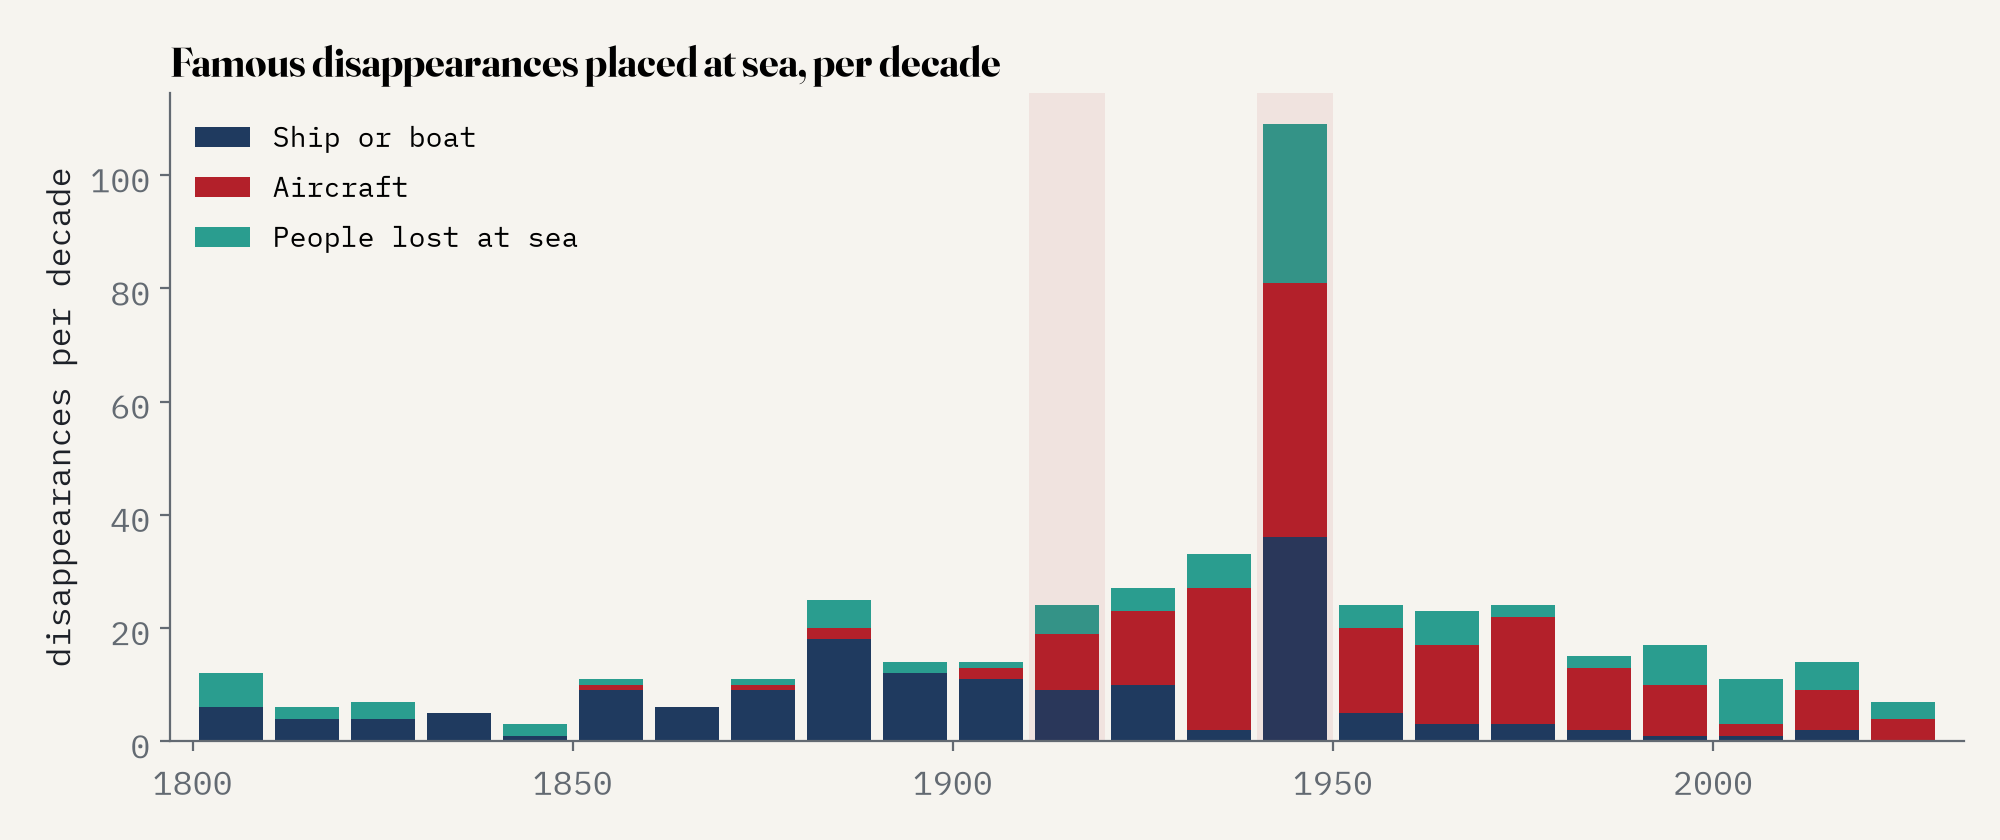
\includegraphics[width=\textwidth]{f_decades.png}\caption{Famous disappearances placed at sea, per decade, by what was lost. Shaded: the decades of the two world wars.}\label{fig:decades}\end{figure}
\begin{figure}[tbp]\centering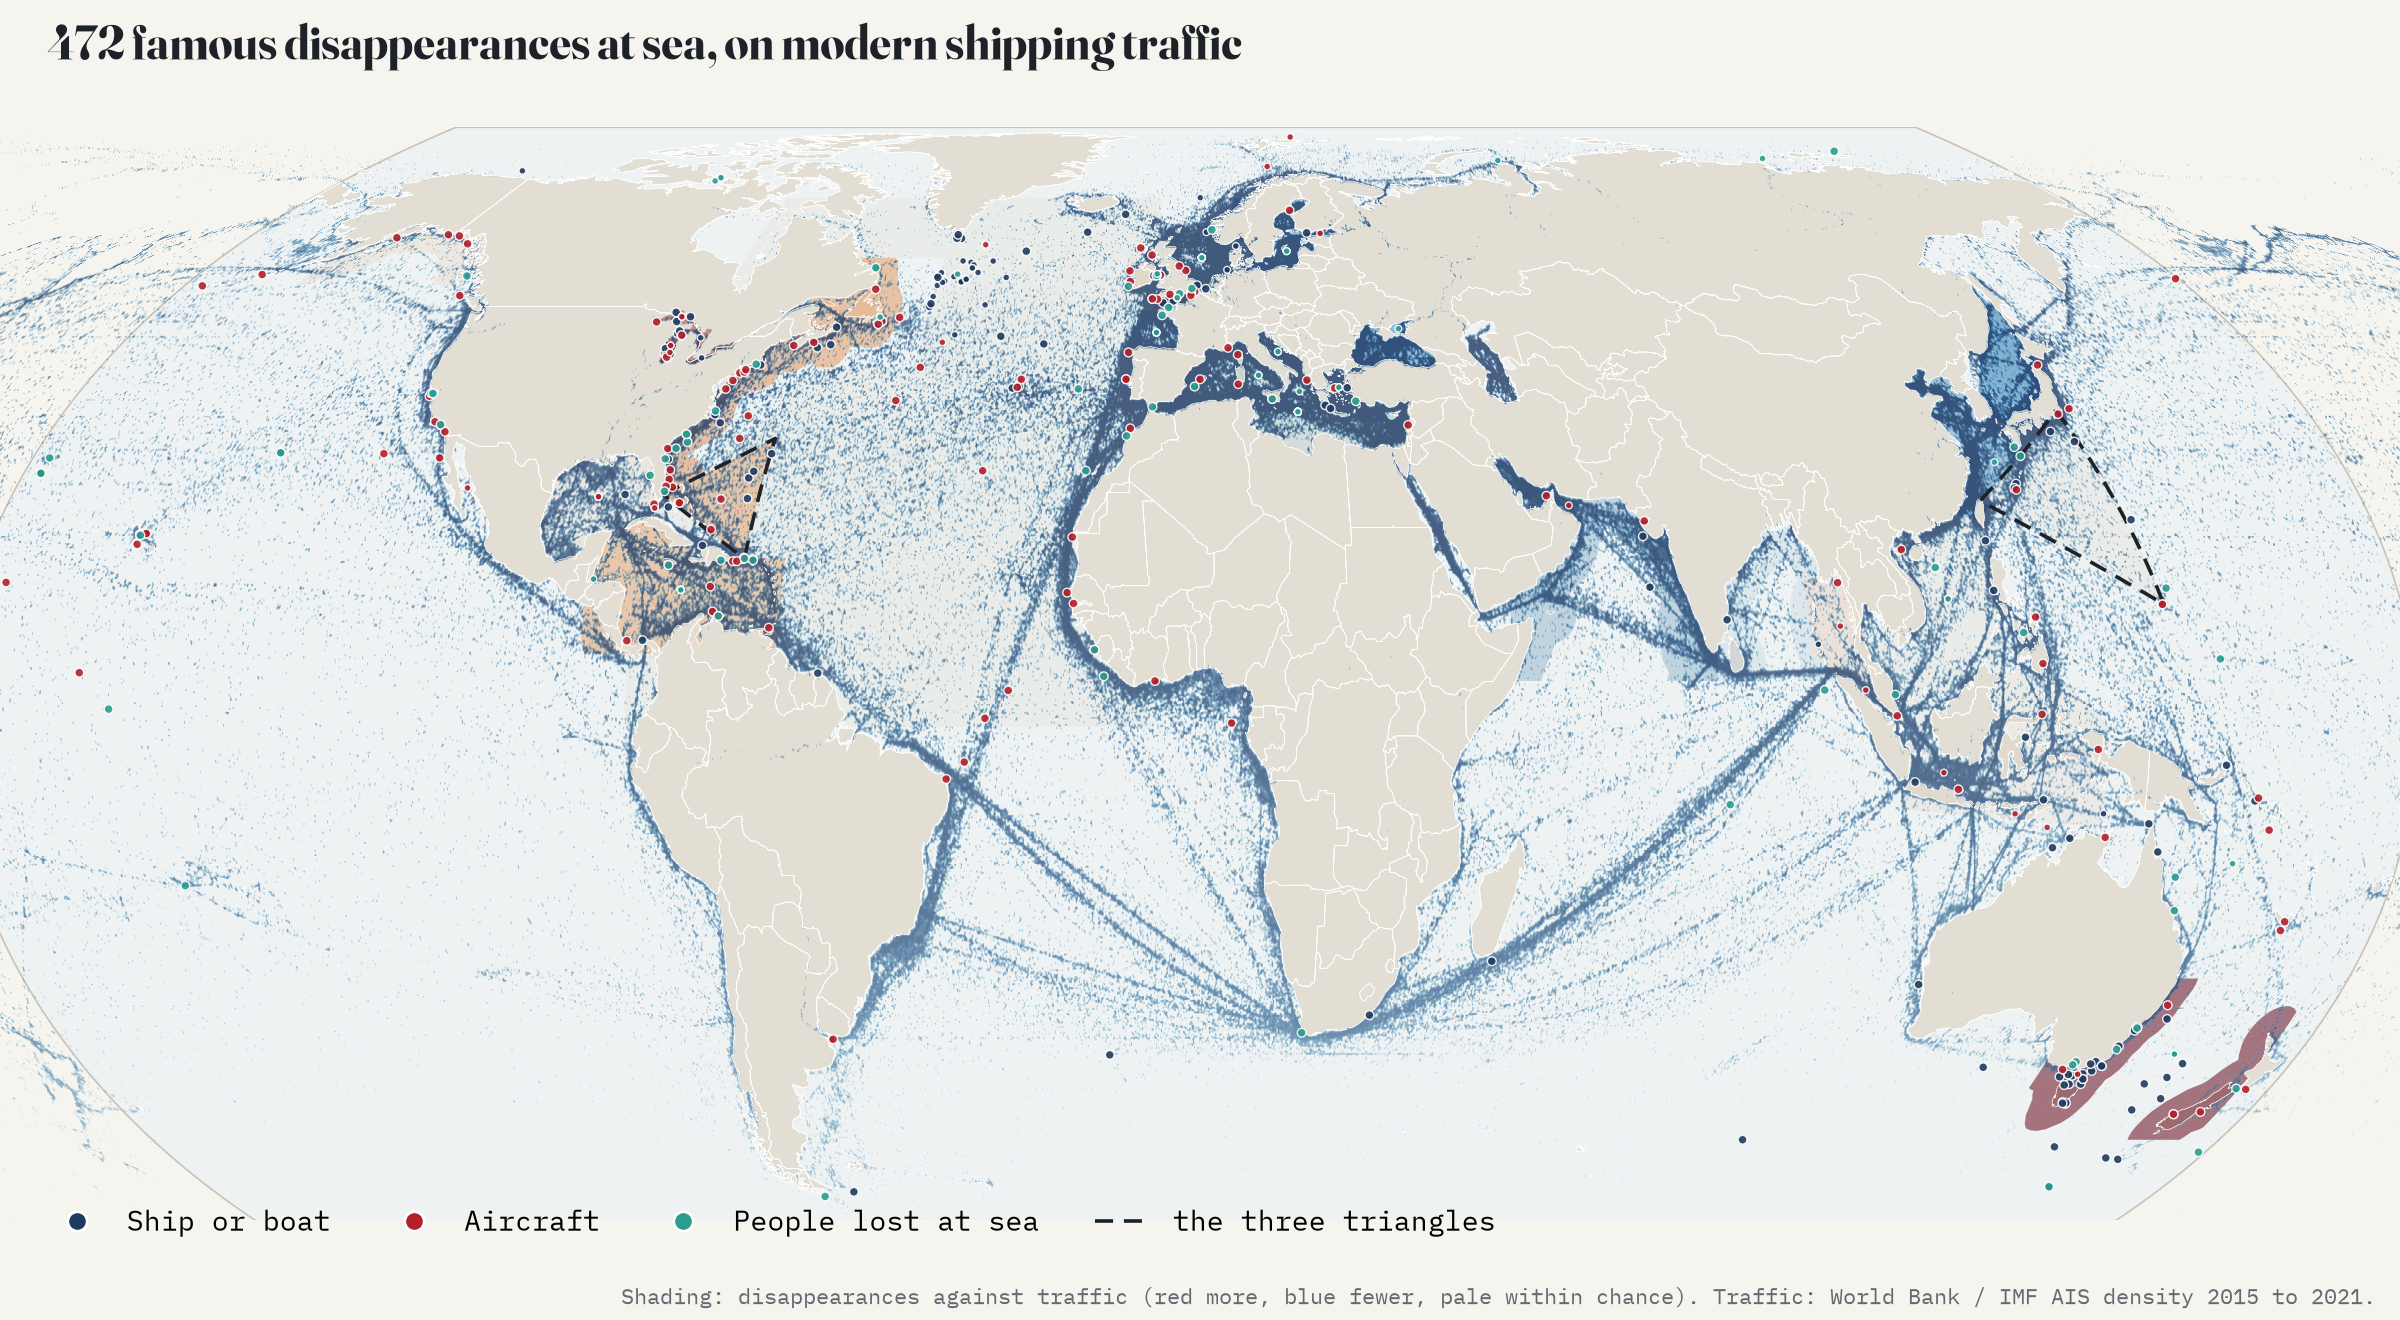
\includegraphics[width=\textwidth]{f_map.png}\caption{The 472 placed disappearances on modern AIS traffic (blue haze), with the three triangles. Sea areas are shaded by test T: red more than expected from traffic, blue fewer, pale within chance. Equal Earth projection.}\label{fig:map}\end{figure}

\subsection{Every sea against its traffic}
Figure~\ref{fig:forest} and Table~\ref{tab:areas} give test T for every area. 7 areas hold clearly more disappearances than their traffic predicts, and 5 clearly fewer: the Mediterranean, the Baltic and the Black Sea, and the East China and Japanese seas. The open North Atlantic (68 against 68.5), the South China Sea and the Gulf of Mexico are as expected. The funnel plot (Figure~\ref{fig:funnel}) shows how far the extreme areas lie beyond chance.

\begin{figure}[tbp]\centering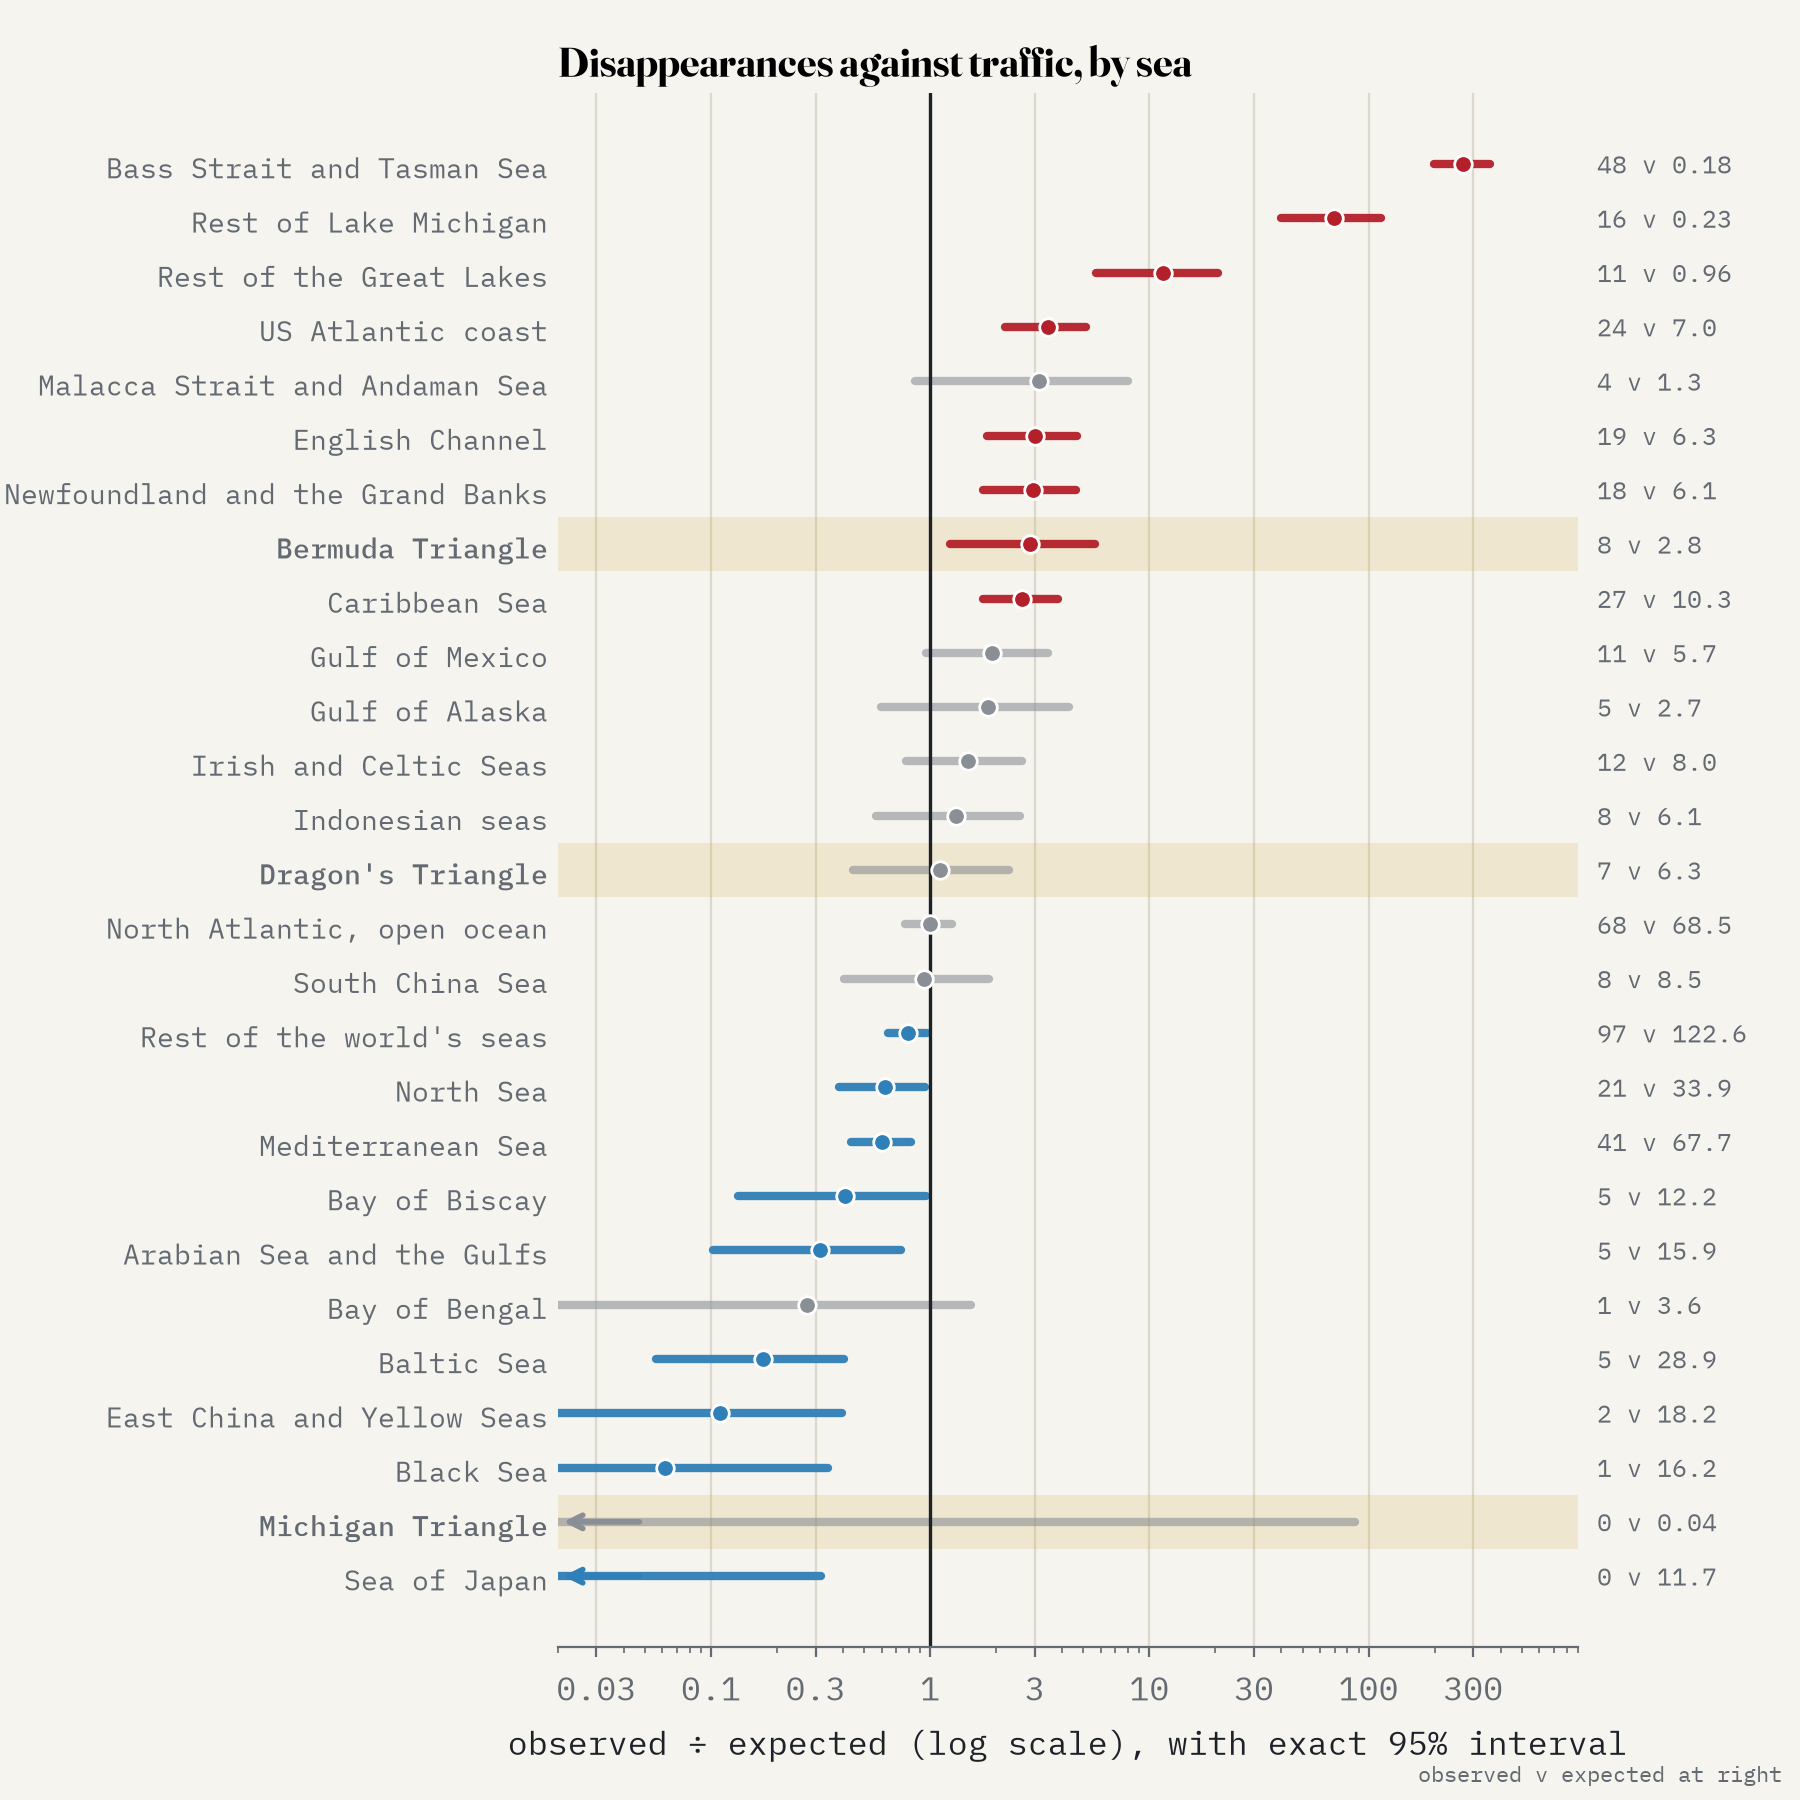
\includegraphics[width=.92\textwidth]{f_forest.png}\caption{Test T: observed disappearances against the number expected from each area's share of AIS traffic, with exact Poisson 95\% intervals (log scale). Shaded rows: the three legendary triangles.}\label{fig:forest}\end{figure}
\begin{figure}[tbp]\centering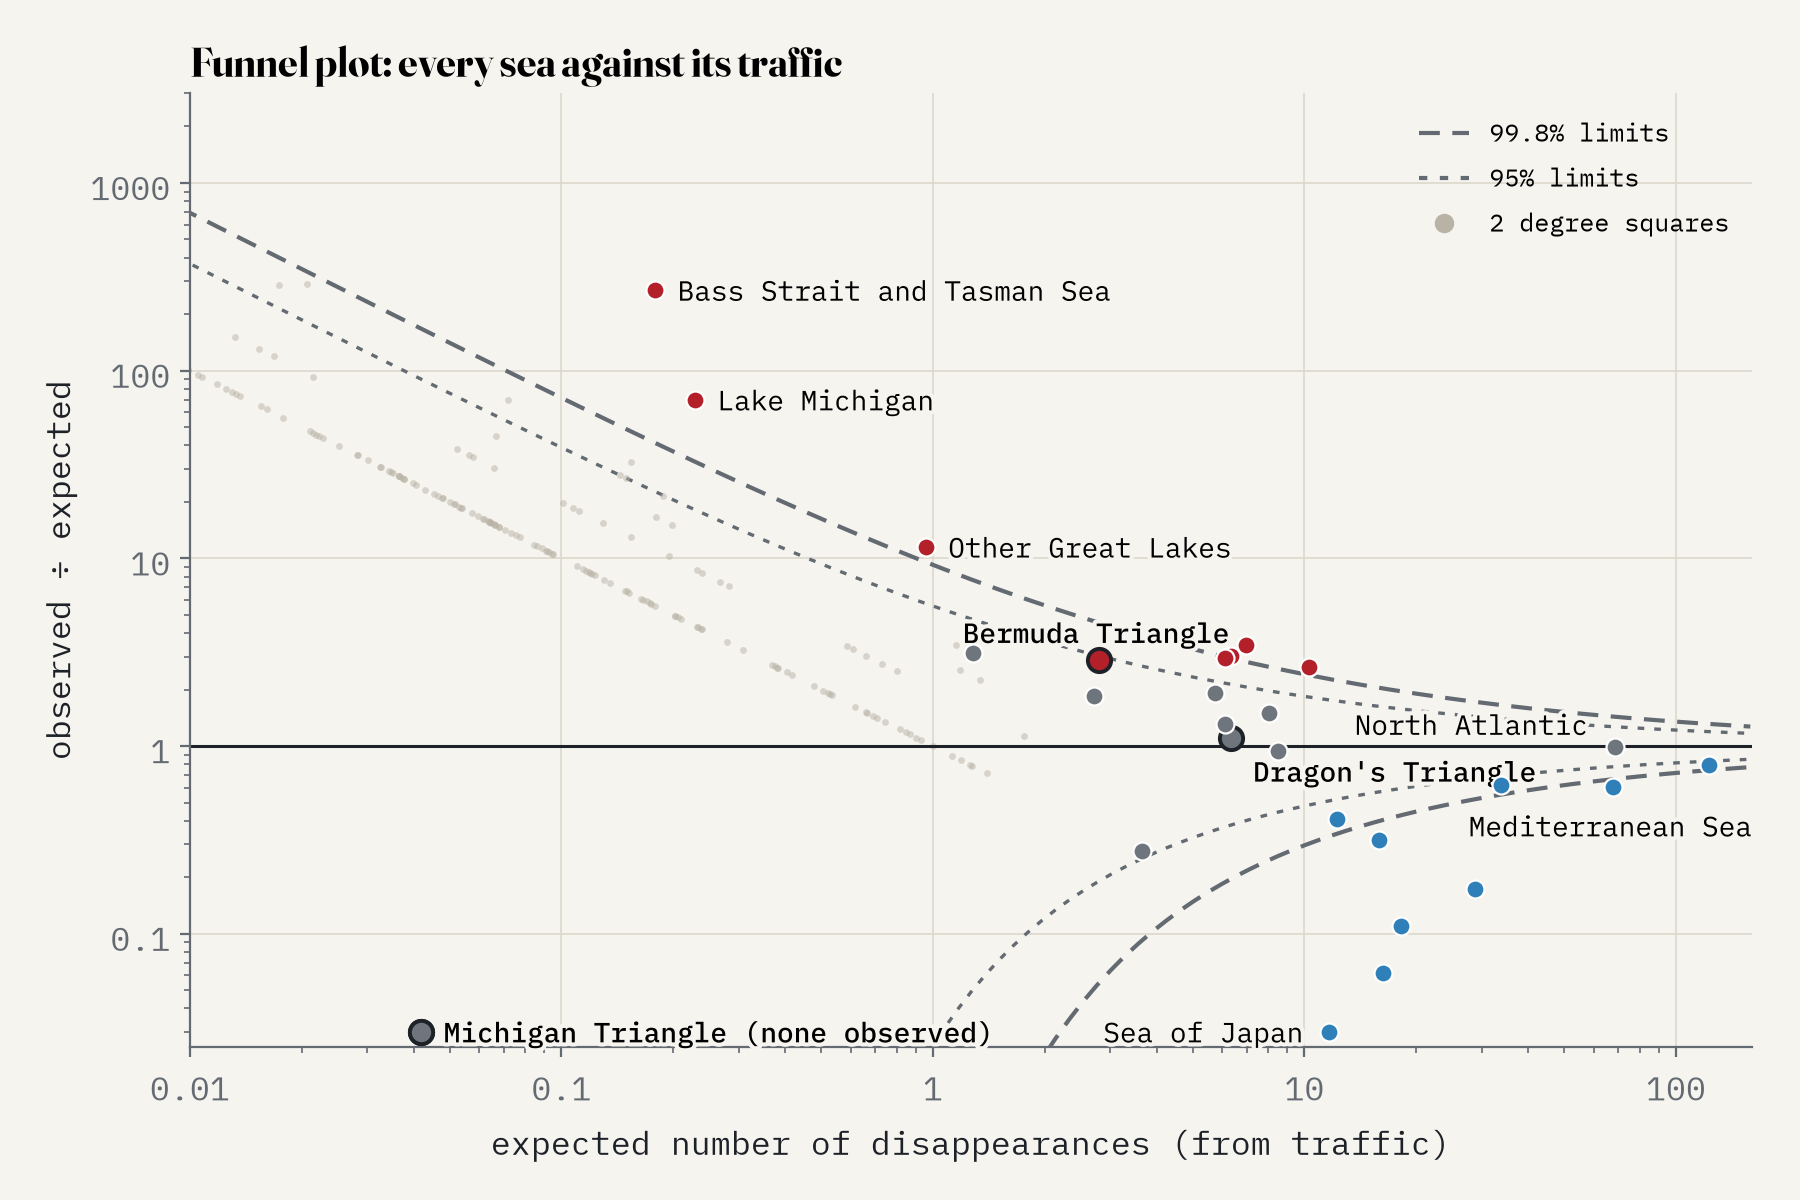
\includegraphics[width=.92\textwidth]{f_funnel.png}\caption{Funnel plot of test T. Points: named areas (coloured by verdict) and 2 degree squares with at least one disappearance (grey). Dashed lines: 95\% and 99.8\% limits if disappearances followed traffic.}\label{fig:funnel}\end{figure}

\begin{table}[tbp]\centering\scriptsize\caption{Test T for every area, sorted by ratio, with test L (ratio against recorded losses of 1800 to 2025) and test M (recorded losses 2000 to 2025, observed / expected).}\label{tab:areas}\begin{tabular}{p{4.0cm}rrrrrlrr}\toprule Area & Traffic \% & O & E & O/E & 95\% interval & Verdict & L: O/E & M: O / E\\\midrule
Bass Strait and Tasman Sea & 0.04 & 48 & 0.18 & 269 & 198 to 356 & clearly more & 34 & 3 / 0.2\\
Rest of Lake Michigan & 0.05 & 16 & 0.23 & 70 & 40 to 113 & clearly more & 7.53 & 0 / 0.2\\
Rest of the Great Lakes & 0.20 & 11 & 0.96 & 11 & 5.74 to 21 & clearly more & 3.50 & 0 / 0.9\\
US Atlantic coast & 1.48 & 24 & 6.98 & 3.44 & 2.20 to 5.12 & clearly more & 1.18 & 94 / 6.4\\
Malacca Strait and Andaman Sea & 0.27 & 4 & 1.28 & 3.12 & 0.85 to 7.99 & as expected & 2.97 & 1 / 1.2\\
English Channel & 1.34 & 19 & 6.33 & 3.00 & 1.81 to 4.69 & clearly more & 0.99 & 3 / 5.8\\
Newfoundland and the Grand Banks & 1.30 & 18 & 6.13 & 2.94 & 1.74 to 4.64 & clearly more & 2.32 & 1 / 5.6\\
Bermuda Triangle & 0.59 & 8 & 2.79 & 2.87 & 1.24 to 5.64 & more (95\%) & 6.48 & 1 / 2.6\\
Caribbean Sea & 2.17 & 27 & 10.27 & 2.63 & 1.73 to 3.83 & clearly more & 3.48 & 5 / 9.4\\
Gulf of Mexico & 1.21 & 11 & 5.73 & 1.92 & 0.96 to 3.43 & as expected & 3.05 & 20 / 5.3\\
Gulf of Alaska & 0.58 & 5 & 2.72 & 1.84 & 0.60 to 4.29 & as expected & 0.14 & 87 / 2.5\\
Irish and Celtic Seas & 1.70 & 12 & 8.03 & 1.50 & 0.77 to 2.61 & as expected & 0.41 & 2 / 7.4\\
Indonesian seas & 1.30 & 8 & 6.12 & 1.31 & 0.56 to 2.58 & as expected & 1.58 & 10 / 5.6\\
Dragon's Triangle & 1.34 & 7 & 6.33 & 1.11 & 0.45 to 2.28 & as expected & 1.29 & 1 / 5.8\\
North Atlantic, open ocean & 14.51 & 68 & 68.47 & 0.99 & 0.77 to 1.26 & as expected & 0.63 & 18 / 62.8\\
South China Sea & 1.80 & 8 & 8.50 & 0.94 & 0.41 to 1.85 & as expected & 0.50 & 21 / 7.8\\
Rest of the world's seas & 25.98 & 97 & 122.60 & 0.79 & 0.64 to 0.96 & fewer (95\%) & 1.30 & 87 / 112.5\\
North Sea & 7.17 & 21 & 33.85 & 0.62 & 0.38 to 0.95 & fewer (95\%) & 0.51 & 13 / 31.1\\
Mediterranean Sea & 14.35 & 41 & 67.75 & 0.60 & 0.43 to 0.82 & clearly fewer & 0.83 & 19 / 62.1\\
Bay of Biscay & 2.59 & 5 & 12.24 & 0.41 & 0.13 to 0.95 & fewer (95\%) & 0.39 & 3 / 11.2\\
Arabian Sea and the Gulfs & 3.36 & 5 & 15.86 & 0.32 & 0.10 to 0.74 & fewer (95\%) & 1.54 & 6 / 14.6\\
Bay of Bengal & 0.77 & 1 & 3.64 & 0.27 & 0.01 to 1.53 & as expected & 0.00 & 3 / 3.3\\
Baltic Sea & 6.11 & 5 & 28.85 & 0.17 & 0.06 to 0.40 & clearly fewer & 0.63 & 8 / 26.5\\
East China and Yellow Seas & 3.86 & 2 & 18.21 & 0.11 & 0.01 to 0.40 & clearly fewer & 0.00 & 18 / 16.7\\
Black Sea & 3.44 & 1 & 16.23 & 0.06 & 0.00 to 0.34 & clearly fewer & 0.41 & 5 / 14.9\\
Michigan Triangle & 0.01 & 0 & 0.04 & 0.00 & 0.00 to 87 & as expected & 0.00 & 0 / 0.0\\
Sea of Japan & 2.47 & 0 & 11.68 & 0.00 & 0.00 to 0.32 & clearly fewer & 0.00 & 4 / 10.7\\
\bottomrule\end{tabular}\end{table}

\subsection{The Bermuda Triangle}
The Bermuda Triangle as drawn covers about 1,136,000 km$^2$ (Wikipedia notes that other authors' versions range from 1.3 to 3.9 million) and carries 0.59\% of the world's AIS traffic. It holds 8 placed disappearances against 2.79 expected: 2.9 times, 95\% interval 1.2 to 5.6, a one-sided probability of 0.008. That is more than chance would usually give, but not beyond the 99.8\% limit. Its four neighbours (the US Atlantic coast, the Caribbean, the Gulf of Mexico and Newfoundland and the Grand Banks) hold 80 against 29.1 (2.7 times, 95\% interval 2.2 to 3.4). Conditioning on the 88 disappearances in the Triangle and its neighbours, the Triangle's share of the group's traffic (8.8\%) predicts 7.7; it holds 8 (binomial $p = 0.51$).

Figure~\ref{fig:tests} shows the Triangle under each test. With the lanes index it is 2.4 times; since 1946, 5 against 0.9, almost all light and military aircraft; for ships alone, 3 against an expected count close to 1, within chance. Against recorded losses it stands out more (6.5 times; without war years 4.2 times), but that comparison is weak here: only 44 recorded wrecks in the Triangle have a position, because ships lost over deep water leave no wreck to plot, and the positioned wrecks of the Atlantic are dominated by wartime sinkings off the American coast. Losses of 2000 to 2025 are as expected (1 against 2.6).

Finally, the legend's own cases mostly lie outside. Of the 14 incidents told in the Wikipedia article, only 2 fall inside the triangle as drawn, both placed at a route midpoint; 8 are within 300 km (Figure~\ref{fig:bermuda}, Table~\ref{tab:famous}). Flight 19, the Cotopaxi and the 1948 DC-3 are placed off Florida's east coast, north of the Miami to Bermuda line; the Marine Sulphur Queen in the Gulf of Mexico; the Star Tiger far out towards the Azores. Kusche made the same observation in 1975 \citep{kusche}.

\begin{figure}[tbp]\centering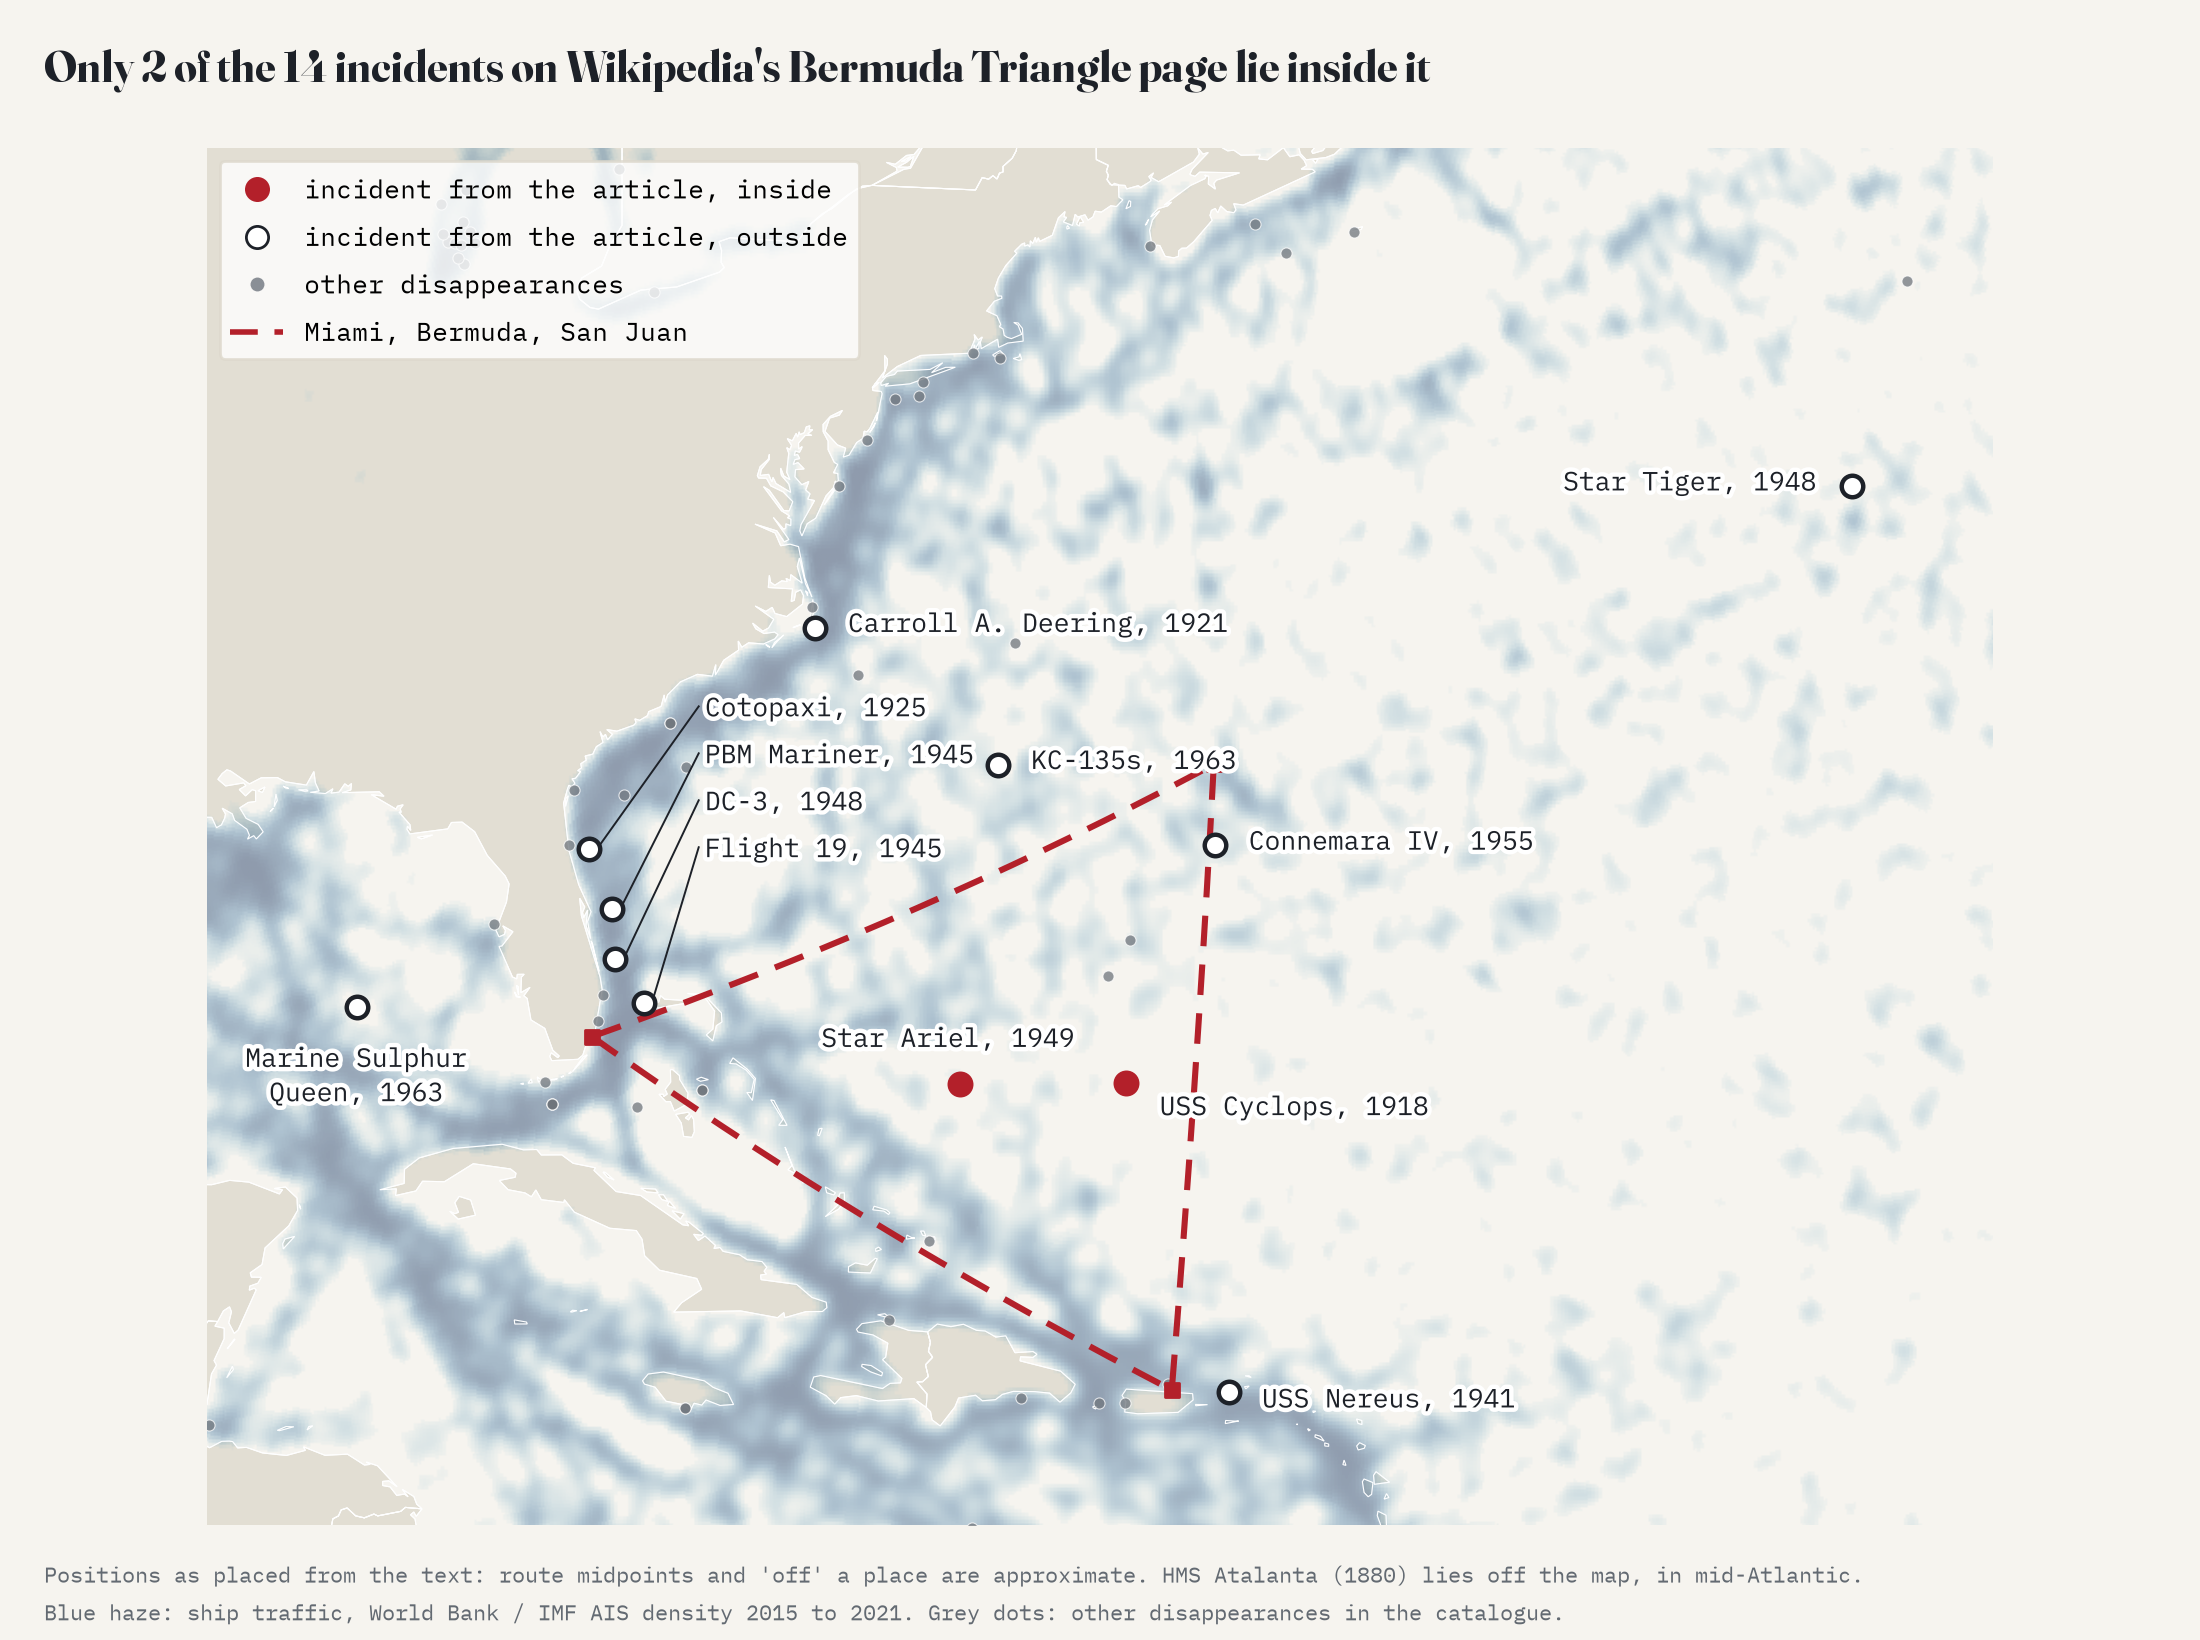
\includegraphics[width=.95\textwidth]{f_bermuda.png}\caption{The incidents of the Wikipedia Bermuda Triangle article as placed from their text (red: inside the triangle; white: outside), other catalogued disappearances (grey) and AIS traffic. Lambert azimuthal equal-area projection centred on 29N, 68W.}\label{fig:bermuda}\end{figure}
\begin{figure}[tbp]\centering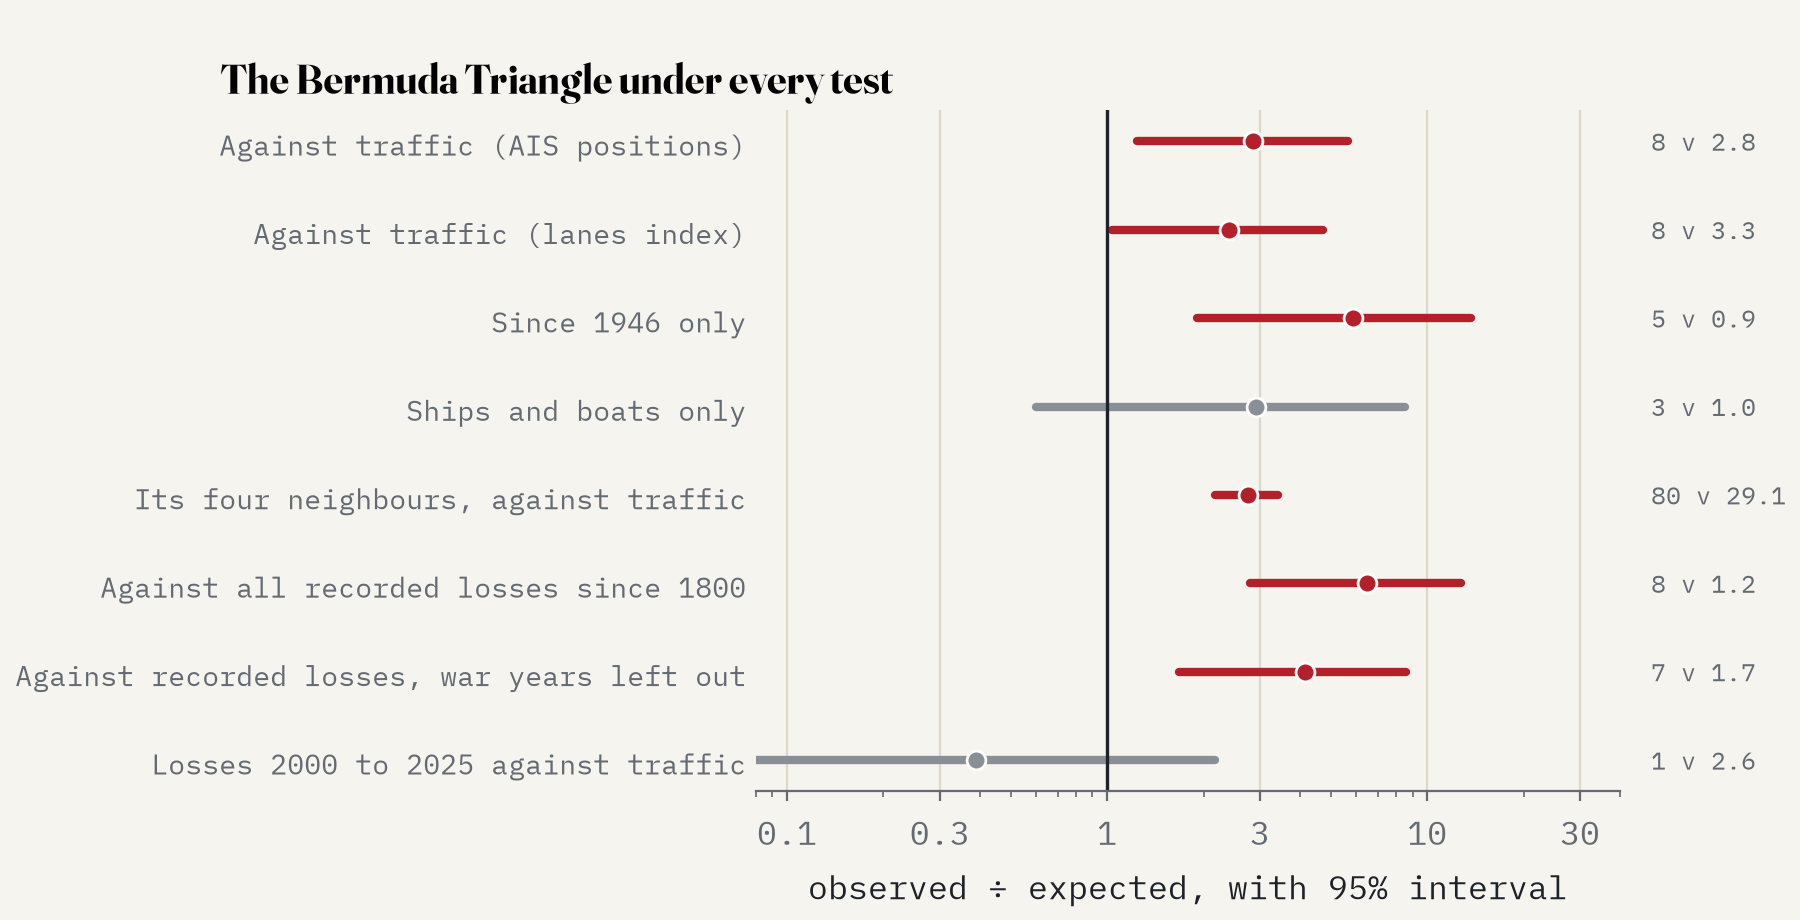
\includegraphics[width=.9\textwidth]{f_tests.png}\caption{The Bermuda Triangle (and its neighbours) under each test, with 95\% intervals. Observed against expected at right.}\label{fig:tests}\end{figure}

\begin{table}[tbp]\centering\small\caption{Incidents told in the Wikipedia article on the Bermuda Triangle: how each was placed and how far outside the Miami, Bermuda and San Juan triangle it falls.}\label{tab:famous}\begin{tabular}{p{6.2cm}rp{3.4cm}r}\toprule Incident & Year & Placed by & Outside by\\\midrule
HMS Atalanta & 1880 & sea area only & 2613 km\\
USS Cyclops & 1918 & route midpoint & inside\\
Carroll A. Deering & 1921 & near a named place & 730 km\\
SS Cotopaxi & 1925 & position given & 433 km\\
USS Nereus & 1941 & near a named place & 139 km\\
USS Proteus & 1941 & sea area only & 786 km\\
Flight 19 & 1945 & near a named place & 34 km\\
PBM Mariner (Flight 19 search) & 1945 & near a named place & 276 km\\
Airborne Transport DC-3 & 1948 & near a named place & 158 km\\
BSAA Star Tiger, with Sir Arthur Coningham & 1948 & route midpoint & 1716 km\\
BSAA Star Ariel & 1949 & route midpoint & inside\\
Connemara IV & 1955 & near a named place & 15 km\\
KC-135 Stratotankers & 1963 & position given & 238 km\\
SS Marine Sulphur Queen & 1963 & position given & 583 km\\
\bottomrule\end{tabular}\end{table}

\subsection{The Dragon's and Michigan Triangles}
The Dragon's Triangle holds 7 disappearances against 6.3 expected (1.1 times, 95\% interval 0.4 to 2.3); 4 are from the Second World War, among them the carrier Shinano. Its most famous case, the research ship Kaiyo Maru No.~5, was destroyed in 1952 by the eruption of the undersea volcano Myojin-sho that she was studying \citep{wikids}. The Michigan Triangle holds none of the catalogue's placed incidents once those placed only as ``Lake Michigan'' are excluded; by my placing, none of the 6 incidents of its article lies inside it, though 4 lie within 50 km. Lake Michigan as a whole, however, is far above its traffic (16 against 0.23, 69.7 times; 43.1 times with the lanes index), as are the other Great Lakes (11 against 0.96).

\subsection{Where the sea really is worse}
Table~\ref{tab:worse} lists the areas beyond the 99.8\% limit, with the likely reasons, and Table~\ref{tab:cells} the most extreme 2 degree squares. Bass Strait and the Tasman Sea lead by far (48 against 0.18; 10.6 times with the lanes index). Most of its incidents are colonial schooners and packets lost between Sydney, Hobart, Launceston and Port Phillip in the 1800s, in a strait swept by westerly gales and crowded with islands and reefs, and they come from one carefully compiled section of the list of missing ships. The Great Lakes follow, for similar reasons: autumn gales and a lake trade a century ago that dwarfed today's. The English Channel's excess is made of early aviators, Battle of Britain pilots and Glenn Miller; the US Atlantic coast's of Cape Hatteras, Gulf Stream storms and light aircraft; the Grand Banks' of fog, ice and pioneer transatlantic flights. Of the 28 flagged squares, 11 are in Bass Strait and the Tasman Sea and 11 owe much to aviation, such as the approaches to Hawaii and the Dole Air Race of 1927. Only 1 is inside the Bermuda Triangle: the Bahamas, with two aircraft.

\begin{figure}[tbp]\centering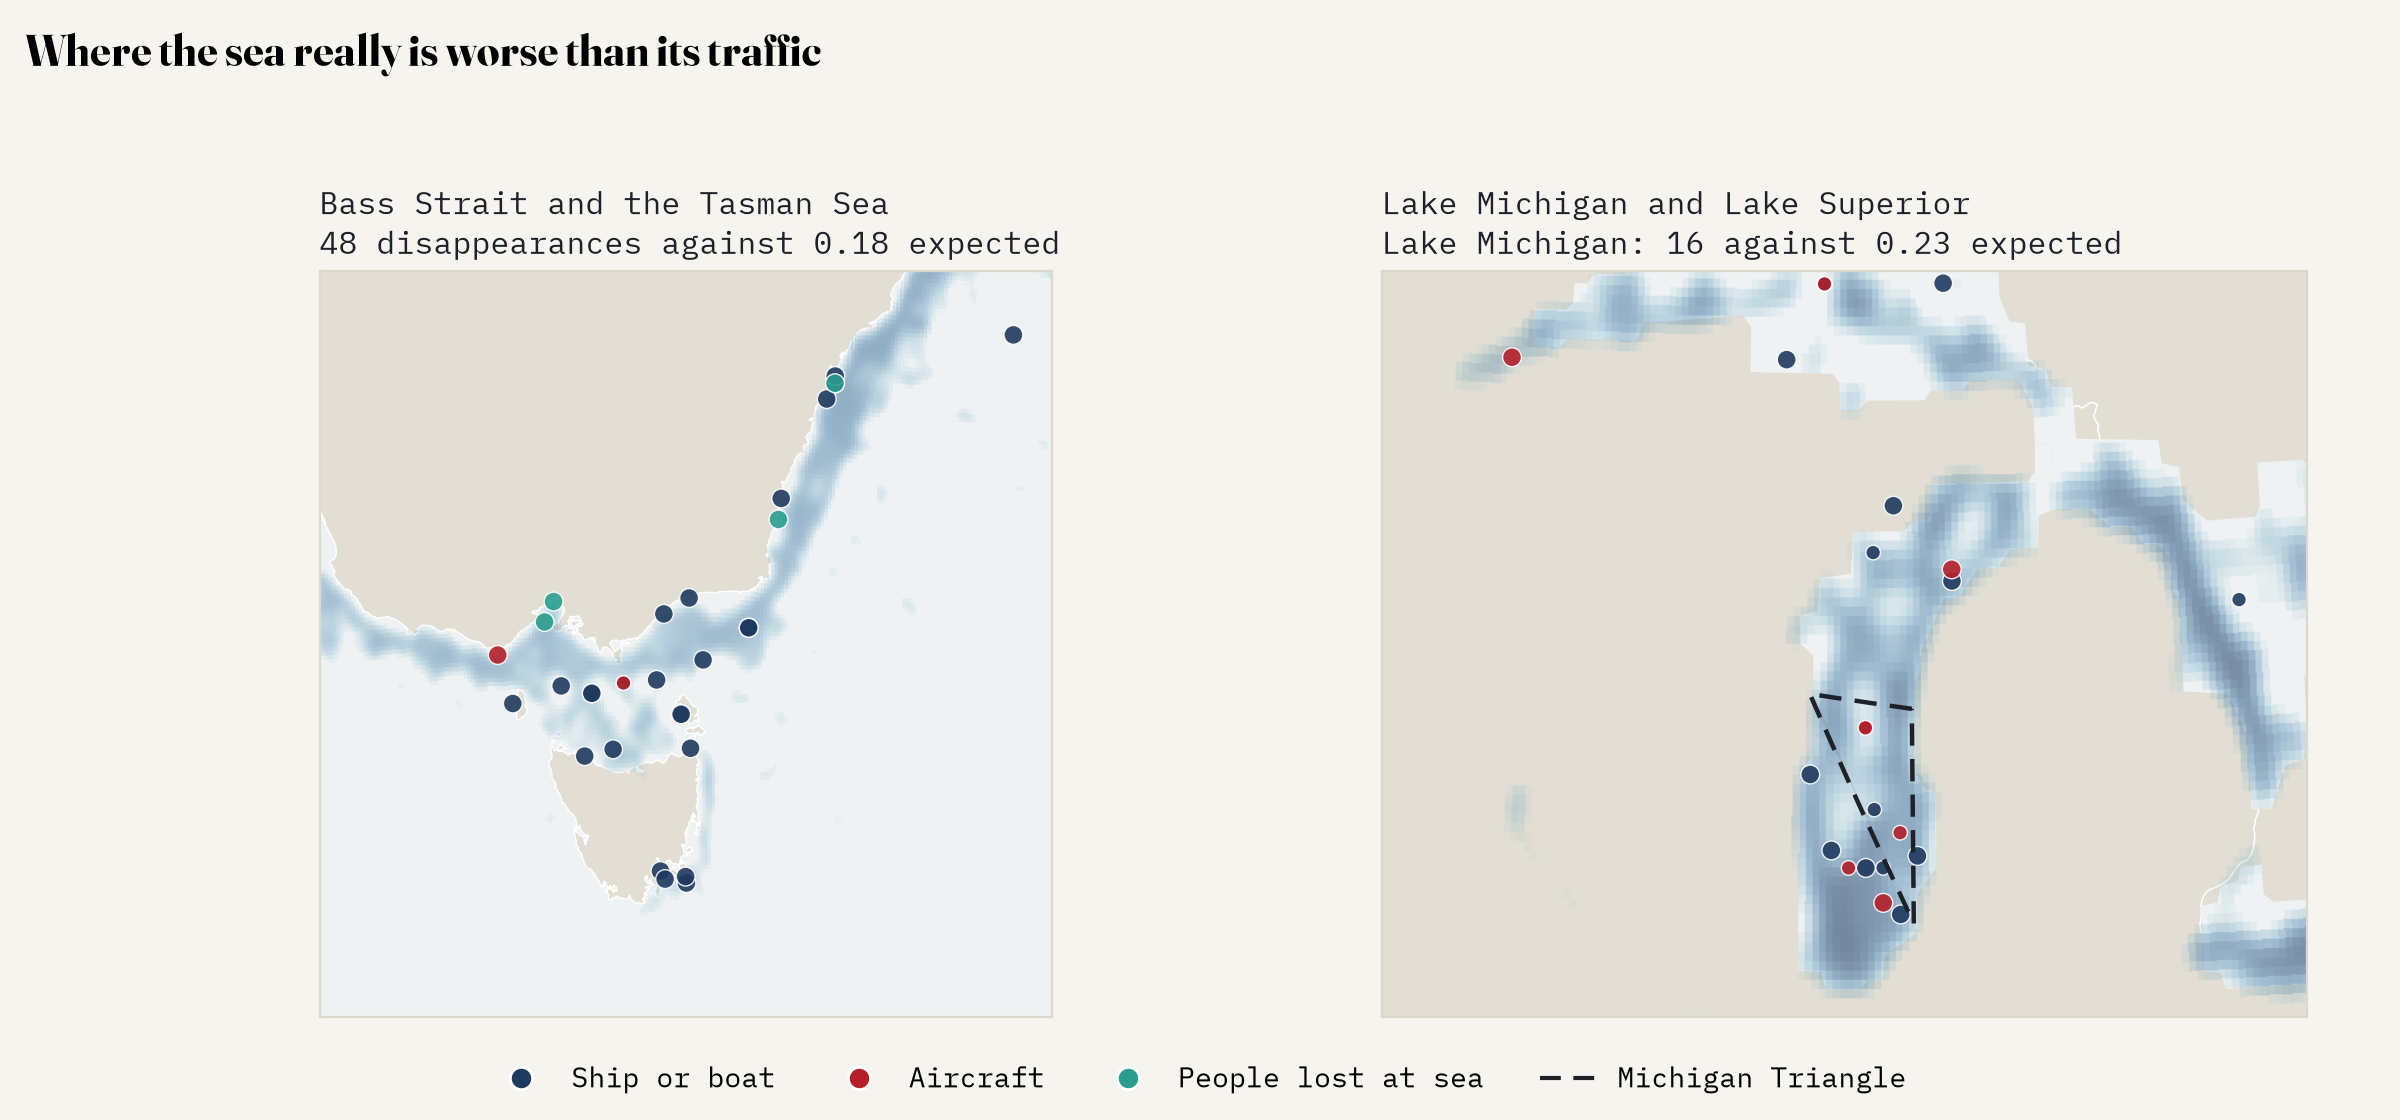
\includegraphics[width=\textwidth]{f_worse.png}\caption{Two seas that really are worse than their traffic: Bass Strait and the Tasman Sea, and Lake Michigan and Lake Superior, with AIS traffic.}\label{fig:worse}\end{figure}

\begin{table}[tbp]\centering\small\caption{Areas clearly worse than their traffic predicts (beyond the 99.8\% funnel limit), with the ratio under the lanes index and the likely reasons.}\label{tab:worse}\begin{tabular}{p{4.6cm}rrrrp{3.6cm}}\toprule Area & O & E & O/E & Lanes O/E & Likely reasons\\\midrule
Bass Strait and Tasman Sea & 48 & 0.18 & 269 & 11 & weather, shoals, reporting\\
Rest of Lake Michigan & 16 & 0.23 & 70 & 43 & weather, history, reporting\\
Rest of the Great Lakes & 11 & 0.96 & 11 & 11 & weather, history\\
US Atlantic coast & 24 & 6.98 & 3.44 & 3.23 & shoals, weather, reporting\\
Caribbean Sea & 27 & 10.27 & 2.63 & 1.96 & weather, history\\
English Channel & 19 & 6.33 & 3.00 & 7.82 & war, aviation, reporting\\
Newfoundland and the Grand Banks & 18 & 6.13 & 2.94 & 3.71 & weather, aviation\\
\bottomrule\end{tabular}\end{table}
\begin{table}[tbp]\centering\small\caption{The 2 degree squares furthest beyond their traffic (at least two incidents and beyond the 99.8\% limit; the 16 most extreme of 28).}\label{tab:cells}\begin{tabular}{p{4.6cm}p{3.2cm}rrp{3.2cm}}\toprule Square & Extent & O & E & Likely reasons\\\midrule
Fiordland, Milford Sound & 43 to 45S, 166 to 168E & 2 & under 0.001 & aviation\\
Hawaii, Oahu and Molokai & 21 to 23N, 156 to 158W & 6 & 0.021 & aviation\\
Bass Strait, west (King Island, Port Phillip) & 39 to 41S, 144 to 146E & 4 & 0.002 & weather, shoals\\
Bass Strait, Tasmania's north coast & 39 to 41S, 146 to 148E & 4 & 0.002 & weather, shoals\\
Bass Strait, east (Furneaux and Kent Groups) & 37 to 39S, 148 to 150E & 4 & 0.003 & weather, shoals\\
Mid-Pacific, Oakland to Hawaii & 29 to 31N, 140 to 142W & 5 & 0.017 & aviation (Dole Air Race)\\
Off Sydney and Botany Bay & 33 to 35S, 150 to 152E & 4 & 0.008 & weather, reporting\\
Macquarie Island & 53 to 55S, 158 to 160E & 2 & under 0.001 & weather\\
South-east Tasmania & 43 to 45S, 148 to 150E & 2 & under 0.001 & weather, shoals\\
Southern Lake Michigan & 41 to 43N, 86 to 88W & 5 & 0.072 & weather, history\\
Hobart and the Derwent & 43 to 45S, 146 to 148E & 2 & under 0.001 & weather, reporting\\
North-east Tasmania & 39 to 41S, 148 to 150E & 2 & under 0.001 & weather, shoals\\
Tasman Sea off New South Wales & 31 to 33S, 154 to 156E & 2 & 0.001 & weather\\
Off Cape Race, Newfoundland & 45 to 47N, 52 to 54W & 5 & 0.154 & weather, aviation\\
Port Phillip Heads & 37 to 39S, 144 to 146E & 2 & 0.001 & weather, reporting\\
Midway & 27 to 29N, 176 to 178W & 2 & 0.001 & war\\
\bottomrule\end{tabular}\end{table}

\subsection{Modern losses against modern traffic}
Test M compares the 433 positioned wrecks of 2000 to 2025 with the AIS traffic of 2015 to 2021 (Figure~\ref{fig:modern}). The areas that stand out are the Gulf of Alaska (34.9 times) and the US Atlantic coast (14.7 times). This too is reporting: 100\% of the Alaskan losses are fishing vessels entered with positions into Wikipedia's monthly shipwreck lists, and 55\% of all positioned losses since 2000 are in North American waters.

\begin{figure}[tbp]\centering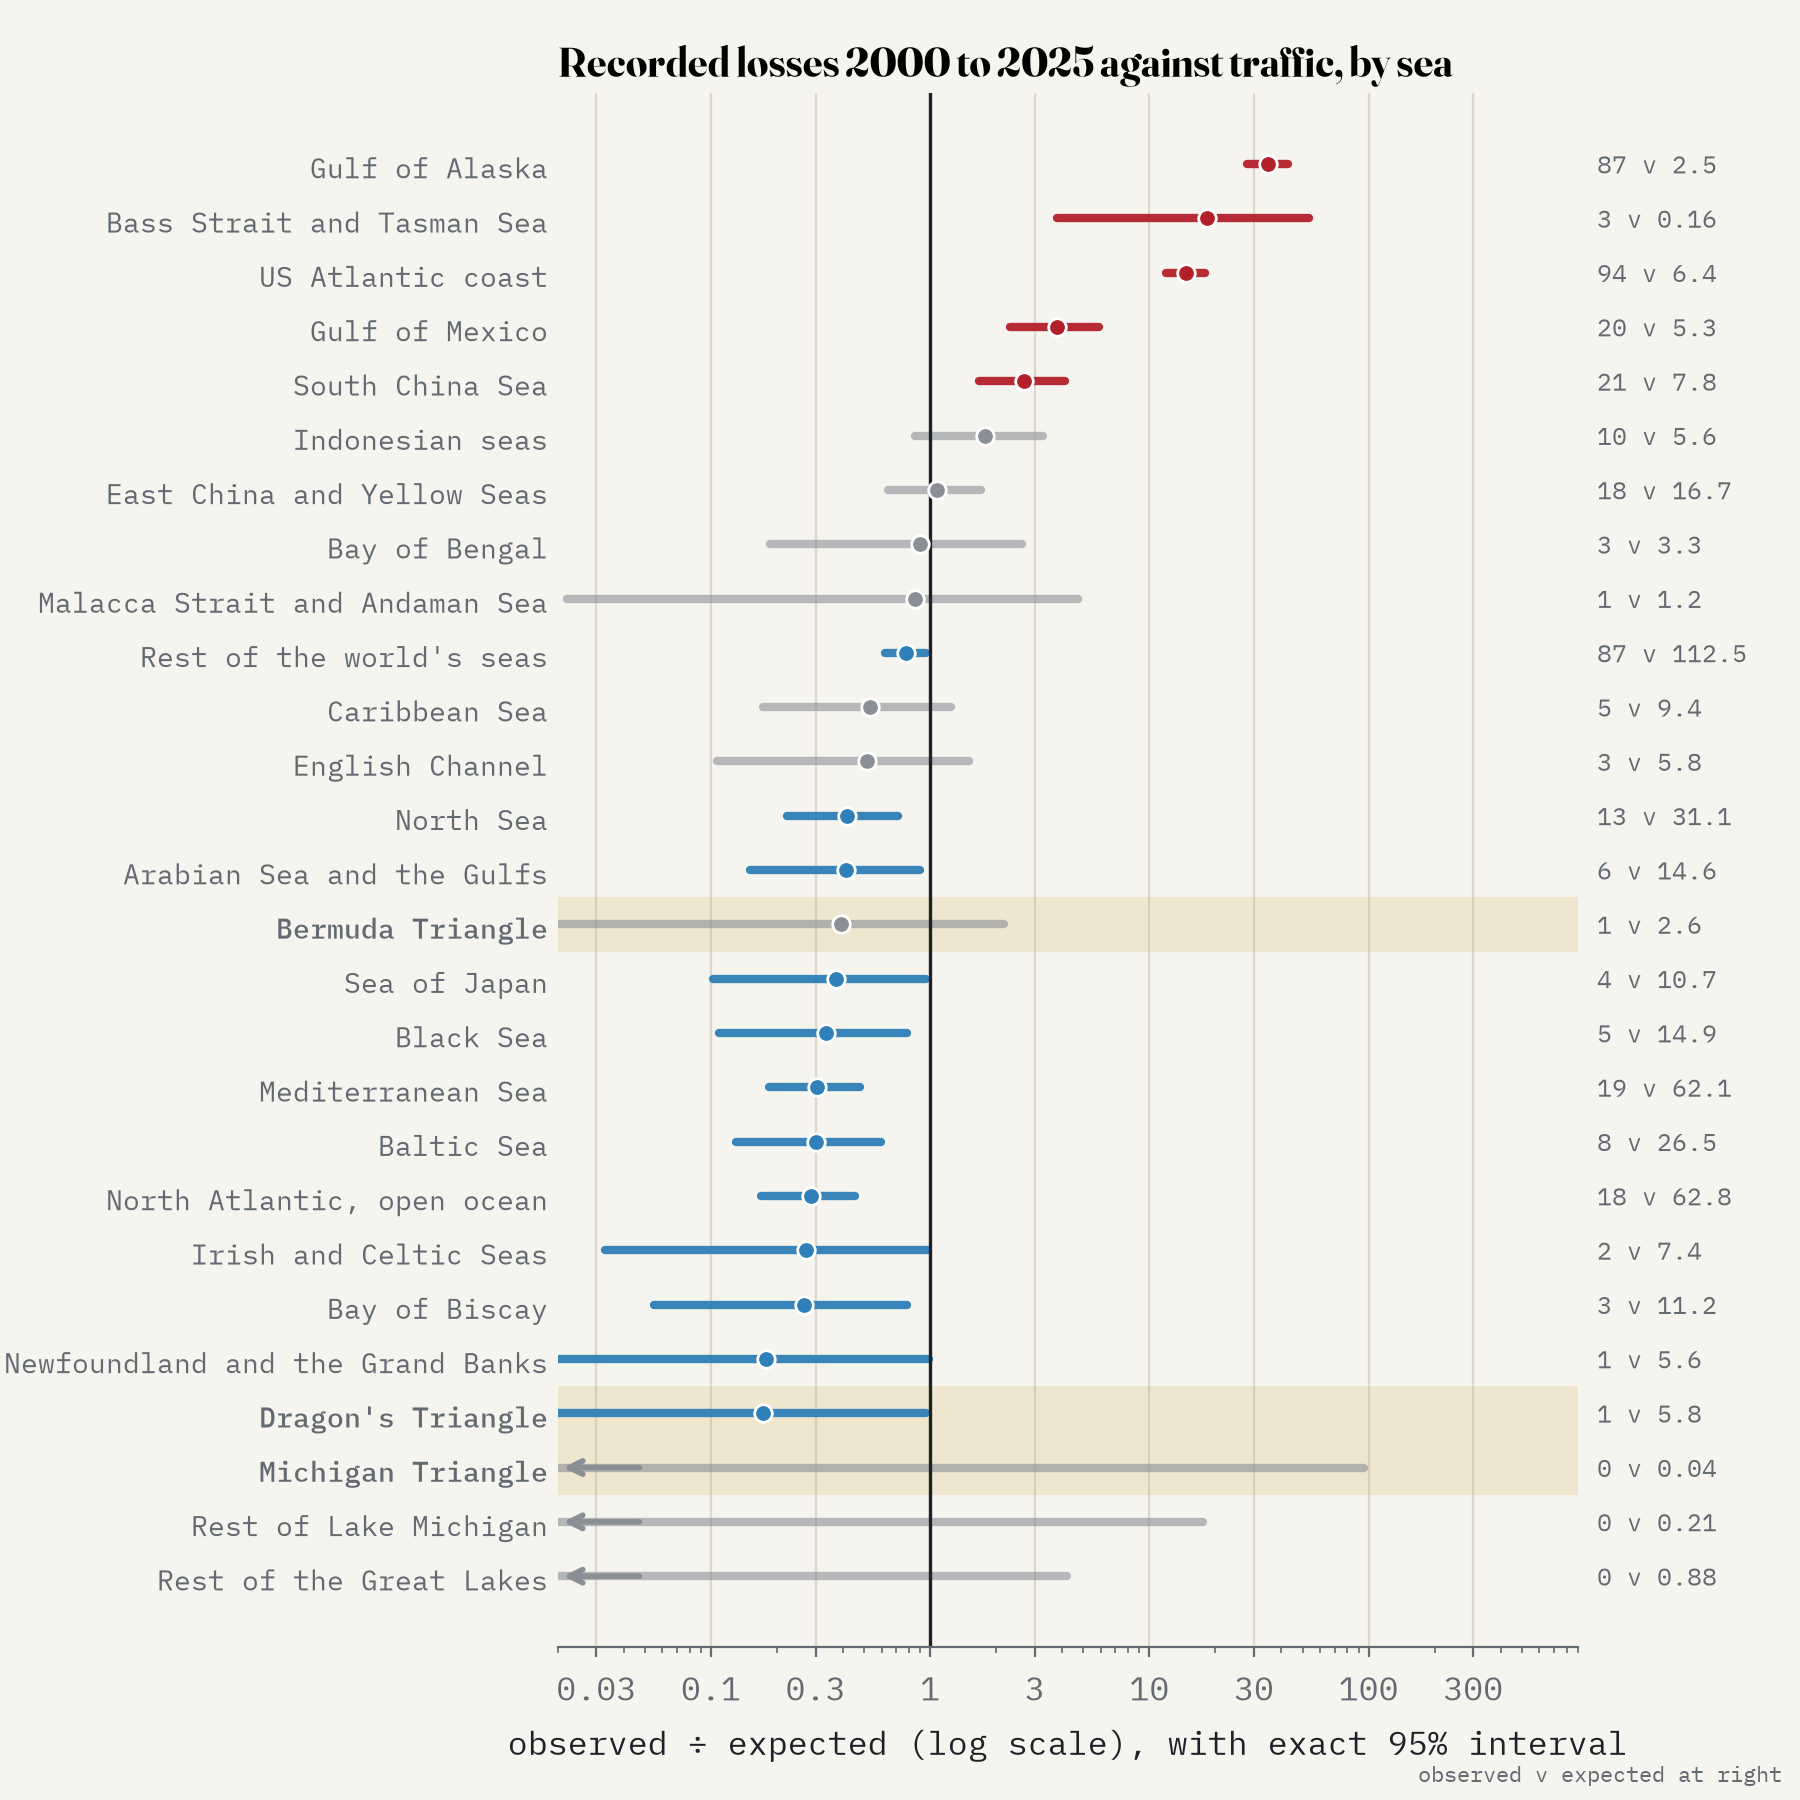
\includegraphics[width=.92\textwidth]{f_modern.png}\caption{Test M: recorded losses of 2000 to 2025 with a position against the number expected from AIS traffic of 2015 to 2021.}\label{fig:modern}\end{figure}

\section{Limitations}
First, the catalogue is of famous disappearances: those that someone wrote about, in English, on Wikipedia. It leans towards the English-speaking world, towards aviation and towards the twentieth century, and its regional sections reflect the energy of particular editors (Australia's colonial losses are an example). Second, many placements are rough: a route midpoint or a sea's representative point can be hundreds of kilometres from the loss, and a different outline for any triangle would change its count. Third, AIS traffic is a modern proxy: it cannot tell us where ships sailed in 1850 or where aircraft flew, and AIS position counts favour coasts with dense receivers, ports and slow vessels, which is why I repeat the tests with a lanes index. Fourth, the recorded-loss denominator is itself biased towards war and towards some countries' records. Fifth, disappearances cluster (one storm, one air race), so Poisson intervals are somewhat too narrow; the conclusions rest on patterns that are large compared with that. Finally, the sea outlines are my own, not the International Hydrographic Organization's.

\section{Conclusion}
The Bermuda Triangle does hold more famous disappearances than its modern traffic predicts, but by the same margin as every sea around it, and most of the incidents that made its name happened outside it. Nothing singles it out. The seas that really are worse than their traffic are less famous and more explicable: stormy straits and lakes that were far busier in the past, routes flown by pioneer aviators, and coasts whose losses were especially well written down.

\section*{Data and code availability}
The interactive map is at \url{https://maps.tristanhotham.com/lost-at-sea/}. Data and code are at \url{https://github.com/Tristan-Hotham/lost-at-sea} and archived with this paper at https://doi.org/10.5281/zenodo.23856868. The disappearance catalogue and the loss table, derived from Wikipedia, are released under CC BY-SA 4.0; other derived data under CC BY 4.0; code under the MIT licence. The AIS density is used under CC BY 4.0 as sums and a rendered image.

\section*{AI statement}
I wrote the text, with drafting and editing assistance from Claude (Anthropic), which also helped prepare the analysis code. I reviewed and checked all text and results.

\begin{thebibliography}{20}
\bibitem[Berlitz(1974)]{berlitz} Berlitz, C. (1974) \emph{The Bermuda Triangle}. New York: Doubleday.
\bibitem[Cerdeiro et al.(2020)]{cerdeiro} Cerdeiro, D. A., Komaromi, A., Liu, Y. and Saeed, M. (2020) World seaborne trade in real time: a proof of concept for building AIS-based nowcasts from scratch. IMF Working Paper 20/57. Washington, DC: International Monetary Fund.
\bibitem[Garwood(1936)]{garwood} Garwood, F. (1936) Fiducial limits for the Poisson distribution. \emph{Biometrika} 28, 437 to 442.
\bibitem[Hotham(2026)]{hotham} Hotham, T. (2026) Shipwrecks of the world, and how many over time: three centuries of recorded losses. Zenodo. \url{https://doi.org/10.5281/zenodo.23850289}
\bibitem[Kusche(1975)]{kusche} Kusche, L. D. (1975) \emph{The Bermuda Triangle Mystery: Solved}. New York: Harper and Row.
\bibitem[Natural Earth(2026)]{naturalearth} Natural Earth (2026) Land, admin 0 countries and populated places. Public domain. \url{https://www.naturalearthdata.com/}
\bibitem[Spiegelhalter(2005)]{spiegelhalter} Spiegelhalter, D. J. (2005) Funnel plots for comparing institutional performance. \emph{Statistics in Medicine} 24, 1185 to 1202.
\bibitem[Wikipedia(2026a)]{wikibt} Wikipedia contributors (2026a) Bermuda Triangle. CC BY-SA 4.0. \url{https://en.wikipedia.org/wiki/Bermuda_Triangle}
\bibitem[Wikipedia(2026b)]{wikids} Wikipedia contributors (2026b) Devil's Sea. CC BY-SA 4.0. \url{https://en.wikipedia.org/wiki/Devil\%27s_Sea}
\bibitem[Wikipedia(2026c)]{wikilm} Wikipedia contributors (2026c) Lake Michigan Triangle. CC BY-SA 4.0. \url{https://en.wikipedia.org/wiki/Lake_Michigan_Triangle}
\bibitem[Wikipedia(2026d)]{wikimships} Wikipedia contributors (2026d) List of missing ships. CC BY-SA 4.0. \url{https://en.wikipedia.org/wiki/List_of_missing_ships}
\bibitem[Wikipedia(2026e)]{wikimair} Wikipedia contributors (2026e) List of missing aircraft. CC BY-SA 4.0. \url{https://en.wikipedia.org/wiki/List_of_missing_aircraft}
\bibitem[Wikipedia(2026f)]{wikipeople} Wikipedia contributors (2026f) List of people who disappeared mysteriously at sea. CC BY-SA 4.0. \url{https://en.wikipedia.org/wiki/List_of_people_who_disappeared_mysteriously_at_sea}
\bibitem[World Bank(2026)]{wbdensity} World Bank (2026) Global Shipping Traffic Density. Data catalogue, dataset 0037580, produced with the IMF from AIS data, January 2015 to February 2021; retrieved 2026. CC BY 4.0. \url{https://datacatalog.worldbank.org/search/dataset/0037580}
\end{thebibliography}
\end{document}
